\documentclass[12pt, a4paper, titlepage]{article}
\usepackage[top=2cm, bottom=2cm, left=2cm, right=2cm]{geometry}
\usepackage{fancyhdr}
\pagestyle{fancy}
\usepackage{graphicx, latexsym}
\usepackage{setspace}
\usepackage{amssymb, amsmath, amsthm}
\usepackage{bm}
\usepackage{epstopdf}
\usepackage[]{hyperref}
\usepackage{xcolor}
\usepackage{apacite}
\usepackage[]{natbib}
\emergencystretch=1em
\hypersetup{
    pdftitle={Research Report},
    pdfauthor={Vera Oosterveen},
    pdfsubject={Master thesis EMOS},
    pdfkeywords={},
    bookmarksnumbered=true,     
    bookmarksopen=true,         
    bookmarksopenlevel=1,       
    colorlinks=true,      
    colorlinks=true,
    citecolor=blue, % changes colors of links in document
    linkcolor=blue,
    urlcolor=blue,           
    pdfstartview=Fit,           
    pdfpagemode=UseOutlines,      
    pdfpagelayout=TwoPageRight
}

\graphicspath{{Images/}} % path to images
\onehalfspacing
\newcommand{\tabitem}{~~\llap{\textbullet}~~} % to insert bullet points in a table


\begin{document}
\title{Detecting incorrect labels in a business register using text classification}
\author{Vera Oosterveen \\   \multicolumn{1}{p{.7\textwidth}}{\centering\emph{Statistics Netherlands \& Utrecht University}}}
\date{\today}
\maketitle

							%%%%%%%%%%
							\begin{abstract}
							The abstract is included in a later stage.
							\end{abstract}
							%%%%%%%%%%


							%%%%%%%%%%
							\section{Introduction}
							\label{section:intro}
							%%%%%%%%%%

National statistical institutes aim to provide official statistics to contribute to the public debate and policy development. Business statistics, such as statistics on turnovers and bankruptcies, give insights into different facets of an economy. These business statistics are often presented by industry, groupings of enterprises with similar economic activities. The classification system for economic activities that is used in the European Union is the NACE (Nomenclature statistique des activités économiques dans la Communauté Européenne). The NACE is a hierarchical classification and contains four-digit codes. National statistical institutes may introduce a fifth digit, as Statistics Netherlands did in the \textit{Standaard Bedrijfsindeling} (SBI).

The NACE codes for Dutch enterprises can be found in the general business register (GBR). An enterprise is described by Statistics Netherlands as a 'statistical unit' and can be a combination of multiple 'legal units'. When a legal unit is registered at the chamber of commerce, the NACE code is determined. 

However, one may question the quality of the NACE codes found in the GBR. \citet{Christensen2008} found that, considering all NACE categories, 18 percent of a sample of Danish firms with at least 5 employees were misclassified. There are no recent quality evaluations available for all NACE codes in the Netherlands. But, for the Dutch car trade sector, with 9 sub-categories, \citet{DeldenScholtusBurger} found that small enterprises (fewer than 10 employees) in certain sectors had a 50 percent probability of misclassification.

The NACE codes in the GBR might be incorrect for several reasons. An incorrect code can be appointed either during registration, if the structure of an enterprise changes over time, or if there are changes in the activity of an enterprise. Changes in economic activity are rarely registered \citep{Christensen2008, DeldenScholtusBurger} since this is not obligatory. The correctness of the NACE codes is of great importance for the quality of the business statistics. Misclassifications in the NACE codes could lead to inaccurate, biased output statistics.

To avoid costly and time-consuming manual checks, national statistical institutes can use additional data sources to validate or supplement the current data. Previous research tried to predict the economic activity codes using text classification approaches. Textual descriptions of the activity \citep{Caterini} or website texts \citep{Roelands, Berardi, Heidi} were deployed to automate the classification of enterprises using machine learning techniques. However, these attempts resulted in low accuracy or high misclassification rates. 

Websites are not necessarily created to describe an economic activity, but are aimed at branding, selling products or selling services. This has two consequences. Firstly, it complicates designing an accurate text classifier. Secondly, the observed label in the GBR might be more informative than the website text. Solely relying on text classification algorithms might not be the optimal strategy to handle the possibly ‘noisy’ labels in the NACE classification.

This research expands the previous work on predicting economic activity based on websites. We do this not by focusing on predicting correct economic activities for enterprises, but by focusing on identifying the incorrectly labeled enterprises. When a machine learning model is not able to predict the correct NACE class of an enterprise based on its website, this does not necessarily indicate that the current label of that enterprise is incorrect. Therefore, we consider the current observed NACE code in the GBR, in addition to a predicted economic activity based on a website. The objective of this study is to develop an approach to point out incorrectly labeled cases in the GBR.

%Knowing which enterprises are likely to have an incorrect NACE code, or which industries have the largest fraction of errors, can contribute to the manual editing process. In the manual editing process, specific enterprises can then be targeted or prioritized.

							%%%%%%%%%%
							\section{Related work}
							\label{section:related}
							%%%%%%%%%%
In the context of text classification and noisy labels, the focus in the literature has mainly been on achieving more accurate classification rates. The effects of noisy labels on commonly-used algorithms (e.g. Support Vector Machines (SVMs), logistic regression, k-nearest neighbours) are well studied \citep{Pech, Nettleton}. In general, the performance of an algorithm decreases when labels in the training data are noisy. However, some algorithms are less influenced by label noise than others \citep{Frenay}. Furthermore, we can distinguish two main approaches to handle label noise \citep{Frenay}: filtering approaches and incorporating a model for the label noise within an algorithm. 

With a filtering approach, the label noise is handled in the data preprocessing stage. Labels that are suspected to be noisy are simply removed from the training set \citep{Brodley}. Removing the suspected noisy cases from the training set may lead to higher classification accuracy, but is problematic when training data is scarce. As pointed out by \citet{Angelova}, good classifiers are needed to detect misclassified cases, and learning from noisy labels results in weak classifiers: a chicken-and-egg dilemma.

Label noise robust variations of common classifiers have been proposed for, among others, logistic regression \citep{Bootkrajang, Rantalainen}), SVMs \citep{Stempfel, Biggio}, and neural-networks \citep{Sigurdsson, Sukhbaatar}). Or, with a Bayesian approach, a prior on the mislabeling probabilities is included in the model (see \citet{Frenay} for references).

Some approaches for incorporating label noise in a model are interesting in particular, since these are more closely related to the current research where we want to point out the noisy labels. A mixture model can be applied to deal with label noise, or to find anomalies or outliers in a dataset. By imposing a mixture model, the population is assumed to consist of multiple subpopulations. Different distributions can thereby be modeled for each subpopulation. \citet{DiZio} and \citet{Eskin} applied such a mixture model. They assumed that the erroneous data and the error-free data came from different distributions. Detecting the noisy cases is then identical to finding out to which distribution a case belongs.

The current study has a similar motivation as the earlier studies of \citet{DiZio, Eskin}, but without assuming a specific distribution for the erroneous and error-free data. In the current research, the erroneous cases will be pointed out based on probability estimates, which is explained in depth in Section~\ref{section:probs}.

Typically, researchers assume a random error pattern for label noise. The reason most research is focused on random noise might be due to the simplicity of random noise \citep{bootkrajang2}. However, non-random noise may be more realistic and is encountered more often in real-world data. Only a few studies addressed the non-random noise. For example, \citet{kolcz} showed that label noise was class-specific in email spam-filtering data. Certain genres of email were much more likely to confuse than others. In the area of speech recognition, \citet{speech} demonstrate that phonetic similarity between the correct word and the recognised word leads to more mislabeling. 

In the current research we will further investigate the non-random label noise. \citet{DeldenScholtusBurger} found that characteristics such as size class and the number of legal units influence the probability of a classification error. Therefore, we assume that the probability of a classification error depends on the characteristics of an enterprise. 

\bigskip

This paper proceeds as follows. In Section~\ref{section:method}, we describe the proposed methodology to find erroneous labeled cases in depth. In turn, we will elaborate on the different experiments that we conduct to test the method (Section~\ref{section:experiments}). 


							%%%%%%%%%%
							\section{Methodology}
							\label{section:method}
							%%%%%%%%%%

In order to point out the erroneous cases, we consider the following four aspects:
\begin{enumerate}
\item The predicted label, based on an enterprises' website,
\item The observed label, as can be found in the GBR,
\item The agreement between the observed label and the predicted label,
\item A non-random probability of an error.
\end{enumerate}

% Predicted label
The predicted label is obtained by fitting a machine learning model, such as a Naive Bayes or SVM. The website texts serve as input for the machine learning model. URLs for websites are obtained from the GBR, or via an external party when a URL was missing in the GBR. The main page is scraped from each website. The text from the main page is tokenized, i.e. split into smaller parts that can serve as features in a machine learning model. 

Moreover, we take note of the observed label. Specifically, we are interested in the agreement between the observed label and the predicted label. An agreement between the two labels leads to more trust in the labels, i.e. a lower probability of an erroneous label. 
We assume that characteristics of an enterprise affect the probability of an error. With a logistic regression model we can relate characteristics of enterprises to the probability of an error. These enterprise characteristics are \textit{the size class}, \textit{the number of legal units that form the statistical unit}, \textit{the number of different activities in the legal units}, \textit{age of the enterprise}, \textit{the NACE codes for the main and secondary economic activity of an enterprise}. The GBR contains these characteristics for all enterprises.
\bigskip

First of all, all mathematical notation will be introduced in the following paragraph. In Section~\ref{section:probs} we explain how we derive the probability of an erroneous label for each case, based on the four aspects mentioned. These probabilities are estimated with an EM algorithm, as is explained in Section~\ref{section:em}.

							%%%%%%%%%
							\subsection{Notation}
							%%%%%%%%%
In this paragraph we introduce the necessary notation.

\textbf{The predicted label.} Let $y^*_i = k$ denote the NACE code predicted by the machine learning model for unit $i$. The input for the machine learning model are the features of the website text, denoted by $\zeta_i$. The parameters of the machine learning model are denoted by $\theta^M$. 

\textbf{The observed label.} The NACE code as found in the GBR is denoted by $\hat{y}_i = h$. 

\textbf{The agreement.} The predicted code $y^*_i = k$ and the observed code  $\hat{y}_i = h$ are compared. Let $a$ denote this agreement, with $a \in \{0,1\}$. Let $a=1$ if the two codes agree and $a=0$ otherwise.

\textbf{The probability of an error.} Finally, we introduce a latent variable, $z_i$, that represents whether a unit's observed code in the GBR is correct or erroneous. Let $z_i = 0$ if the code in the GBR is the true code and $z_i = 1$ when the code in the GBR is incorrect. The variable $z_i$ can be modeled as a function of enterprise characteristics using logistic regression. The probability of an error, $P(z_i = 1)$, may depend on enterprise characteristics, which are denoted by $u_i$. Let $\theta^R$ denote the parameters of the logistic regression model. The full set of model parameters is therefore $\theta \in \{ \theta^M, \theta^R\}$. 

Throughout this paper we assume that each unit has a single true (unknown) NACE code which is considered as fixed. That is, the NACE code that is derived when all economic activity information is available without error and the rules to derive a NACE code are applied correctly.

					%%%%%%%%%%
					\subsection{Deriving the probability of being erroneous}
					\label{section:probs}
					%%%%%%%%%%

We are interested in the probability that a unit is incorrectly labeled, given the agreement between observed and predicted code, enterprise characteristics, features derived from the website text, and the model parameters. This is defined as $\tau_i$:

						\begin{equation} \label{eq:1}
\tau_i(\hat{a}_i = a) \equiv P(z_i = 1 | \hat{a}_i = a, \hat{y}_i = h, \zeta_i, u_i, \theta).
						\end{equation}

To find a probability for Equation~\ref{eq:1}, we use \textit{Bayes' Theorem} with multiple conditions:

						\begin{equation*} \label{eq:bayes}
P(A | B, C) =  \frac{P(A | C) P(B | A, C)}{P(A|C)P(B|A,C) + P(A^C|C)P(B|A^C, C)}   .
						\end{equation*}

Substituting elements of Equation~\ref{eq:1} into Bayes' Theorem gives: 
%A for $z_i = 1$, B for $\hat{a}_i = 1$, and C for $\hat{y}_i = h, \zeta_i, u_i, \theta$ gives:

						\begin{equation}\label{eq:2}
\tau_i(\hat{a}_i = 1) = P(z_i = 1 | \hat{a}_i = 1, \hat{y} = h, \zeta_i, u_i, \theta) = 
						\end{equation}

						\begin{equation}\label{eq:3}
\frac{P(z_i = 1|\hat{y}_i = h, \zeta_i, u_i, \theta)P(\hat{a}_i=1|z_i=1, \hat{y}_i = h, \zeta_i, u_i, \theta) }
{\sum_{z=0,1}P(z_i=z|\hat{y}_i = h, \zeta_i, u_i, \theta) P( \hat{a}_i=1|z_i=z, \hat{y}_i = h, \zeta_i, u_i, \theta  )} .
						\end{equation}


The first term in Equation~\ref{eq:3}, $P(z_i = 1|\hat{y}_i = h, \zeta_i, u_i, \theta)$, represents the probability of an error given the observed label, features of the website, enterprise characteristics, and the model parameters. Before, we already stated why the enterprise characteristics influence the error-probability. Furthermore, we assume that the probability of an error does not directly depend on the features of the website or on the parameters of the machine learning model. However, the website text (and therefore the features derived from the website text) can indirectly influence the probability of an error. That is, units for which it is more difficult to derive the NACE code may also have more vague website texts, or websites with less text. The indirect effect of the website text can be captured in $u_i$; we include for instance the number of words in the website text in $u_i$. Given these assumptions, we obtain the probability of an error, which we denote as $\pi_i$:

						\begin{equation}\label{eq:pi4}
\pi_i \equiv P(z_i = 1|\hat{y}_i = h, \zeta_i, u_i, \theta = P(z_i = 1|\hat{y}_i = h, u_i, \theta^R) .
						\end{equation} 

The term $P(\hat{a}_i=1|z_i=1, \hat{y}_i = h, \zeta_i, u_i, \theta)$ in Equation~\ref{eq:3} stands for the probability of agreement between the observed and predicted codes, given that the label is incorrect. Let us define this probability $\gamma$ and assume this is a small probability. There is a small probability that a NACE code changes in a given period, when the code before and after was incorrect \citep{VanDelden}. Therefore, an initial estimate for $\gamma$ can be obtained as the fraction of incorrect cases among all cases where the predicted NACE code $y^*_i$ and the observed NACE code $\hat{y}_i$ agree:

						\begin{equation}\label{eq:gamma5}
\hat{\gamma} = \sum_{i} z_i \hat{a}_i / \sum_{i} z_i.
						\end{equation} 


Furthermore, we consider the probability of an agreement, given that the label is correct: $P(\hat{a}_i=1|z_i=0, \hat{y}_i = h, \zeta_i, u_i, \theta)$. This probability can be estimated for the probability that $y^*_i = h$ based on the fitted machine learning model. Therefore, $P(\hat{a}_i=1|z_i=0, \hat{y}_i = h, \zeta_i, u_i, \theta) = P(y^*_i = h | z_i = 0, \zeta_i, u_i, \theta^M)$. 


Equation~\ref{eq:3} can now be rewritten as:
						\begin{equation}\label{eq:6}
\frac{\pi_i \gamma}{(1-\pi_i)P(y^*_i = h | z_i = 0, \zeta_i, u_i, \theta^M) + \pi_i \gamma  }.
						\end{equation}

The equation above implies that when $\gamma$ and $\pi_i$ are small, and the machine learning model predicts the right NACE code with a high probability, the probability of an erroneous case is low.

Likewise, there is the probability of an erroneous label, $\tau_i$, when there is disagreement between the observed label $\hat{y}_i$ and the predicted label $y^*_i$:

						\begin{equation}\label{eq:7}
\tau_i(\hat{a}_i = 0) = (z_i = 1 | \hat{a}_i = 0, \hat{y} = h, \zeta_i, u_i, \theta) = 
						\end{equation}

						\begin{equation}\label{eq:8}
\frac{P(z_i = 1|\hat{y}_i = h, \zeta_i, u_i, \theta) P(\hat{a}_i=0|z_i=1, \hat{y}_i = h, \zeta_i, u_i, \theta) }
{\sum_{z=0,1}P(z_i=z|\hat{y}_i = h, \zeta_i, u_i, \theta) P( \hat{a}_i=1|z_i=z, \hat{y}_i = h, \zeta_i, u_i, \theta  )} =
						\end{equation}

						\begin{equation}\label{eq:9}
\frac{\pi_i P(\hat{a}_i=0|z_i=1, \hat{y}_i = h, \zeta_i, u_i, \theta) }
{(1-\pi_i)P(\hat{a}_i = 0 | z_i = 0, \zeta_i, u_i, \theta) + \pi_i P(\hat{a}_i = 0 | z_i = 1, \zeta_i, u_i, \theta) } .
						\end{equation}

The term $P(\hat{a}_i= 0|z_i = 1, \hat{y}_i = h, \zeta_i, u_i, \theta)$ represents the probability that the observed NACE code and predicted code disagree, given that the label is incorrect. This can be estimated by $1-\gamma$.

The term $P(\hat{a}_i = 0 | z_i = 0, \zeta_i, u_i, \theta)$ represents the probability of disagreement, given that the label is correct. This probability is equal to $1 - P(\hat{a}_i = 0 | z_i = 0, \zeta_i, u_i, \theta) = 1 - P(y^*_i = h | z_i = 0, \zeta_i, u_i, \theta^M)$. 

Equation~\ref{eq:9} can be rewritten as:

						\begin{equation}\label{eq:10}
\frac{\pi_i (1-\gamma)}{(1-\pi_i)(1-P(y^*_i = h | z_i = 0, \zeta_i, \theta^M)) + \pi_i (1-\gamma)}   .
						\end{equation}


This implies that the probability of an erroneous label is large when, according to the machine learning model, it is likely that the NACE code of unit $i$ differs from the code that is observed in the GBR.

In summary, Equation~\ref{eq:6} or Equation~\ref{eq:10} is used to estimate the probability of a case being erroneous. If this probability is greater than 0.5 for a unit, this unit is considered erroneous and we set $z_i = 1$. If the probability of being erroneous is smaller than 0.5, a unit is seen as correct and, therefore, $z_i=0$.


					%%%%%%%%%%
					\subsection{Estimation using the EM algorithm}
					\label{section:em}
					%%%%%%%%%%

The model parameters are estimated with the Expectation Maximization (EM) algorithm. The EM algorithm can be used for maximum likelihood estimation in incomplete data problems \citep{Rubin}. In our case, the data are seen as incomplete because the values for the latent variable $z_i$ are missing for a part of the data. The EM algorithm provides us with a way of estimating the values for $z_i$.

The EM algorithm consists of an Expectation step (E-step) and a Maximization step (M-step). As input, the model requires a labeled set. This is a set of data for which $z_i$ is known. The part where $z_i=0$ is the gold set: a set where the labels are correct almost certainly. In the real-world GBR data, the large, influential enterprises can be used as the gold set. The large enterprises are checked manually by Statistics Netherlands. The other part of the labeled set is the false set. Here, $z_i = 1$ and this (artificial) set represents the prior knowledge about the errors in the data. This part is needed to initiate the logistic regression model, since both correct and incorrect examples have to be provided to estimate parameters. 

The EM algorithm needs starting values to initialize the model, meaning we provide an initial value for all units for $z_i$. These starting values can be derived in different ways, based on the labeled set. Then, the algorithm estimates model parameters for the machine learning model, $\theta^M$, and the logistic regression model, $\theta^R$, based on the values of $z_i$. Only the units with $z_i=0$ are used for training the machine learning model. In the subsequent E-step the values of $\tau_i$ are estimated given the model parameters $\theta$. When iterating, the models are retrained in the M-step. A difference with the previous M-step is that the estimates for $\tau_i$ serve as weights while training the machine learning model. In other words, $\tau_i$ represents the contribution of a unit to the parameter estimation in the machine learning model. The algorithm is presented in Table~\ref{tab:table1}.

\begin{table}
						\caption{\label{tab:table1}The EM algorithm.}
\centering 
\begin{tabular}{ll}
\hline
\textbf{Input} & A labeled set consisting of a gold set ($z_i = 0$) and a false set ($z_i = 1$)
\\ \hline
\textbf{Initialize} & Estimate $\tau_i$ for all units in the population                                                                                              \\ \hline
\textbf{M-step}     & \begin{tabular}[c]{@{}l@{}}\tabitem Train a machine learning model \end{tabular} \\
                    & \begin{tabular}[c]{@{}l@{}}\tabitem Fit a logistic regression model \end{tabular} \\
                    & \tabitem Estimate $\gamma$                                                                                                                              \\ \hline
\textbf{E-step}     & Re-estimate $\tau_i$ according to Equation~\ref{eq:6} and \ref{eq:10}.                                                                                \\
                    & If $\tau_i > .5$ set $z_i = 1$ and $z_i = 0$ otherwise                                                                                         \\ \hline
\textbf{Iterate}    & \begin{tabular}[c]{@{}l@{}}Repeat the E- and M-step until the changes in $\tau_i$ are smaller than 1e-9.\end{tabular}   
\end{tabular}
\end{table}

%% INPUT!!

%% labeled set

It is known that a different set of starting values might lead to a different solution \citep{Shireman}. Therefore, we will try several sets of starting values. In order to select the optimal starting values for the EM algorithm, we use the log-likelihood of the labeled set. Within the labeled set, there is a part with $z_i = 1$ and a part with $z_i = 0$. For the part with $z_i = 1$ we are interested in the estimated probabilities for $\tau_i$. These probabilities are ideally close to 1. For the part of the labeled set where $z_i = 0$, we do know the true NACE code for unit $i$. We want to extract the probability that the machine learning model predicts this true NACE code. Preferably, this probability is close to 1.
The log-likelihood is then given by:

						\begin{equation}\label{log}
log \sum_i z_i \tau_i + \sum_k (1-z_i)I(y_i = k)\hat{P}(y_i=k),
						\end{equation}
						

where the indicator $I(y_i = k) = 1$ if the label is correct, and $0$ otherwise, so that we sum the predicted probabilities of the correct labels.


							%%%%%%%%%%
							\section{Experiments}
							\label{section:experiments}
							%%%%%%%%%%

This section describes the experimental evaluation of the method. The goal is to investigate under which circumstances the method is (not) able to find the erroneous cases. Section~\ref{section:synthdata} describes how a synthetic dataset is created. The different experimental settings are explained in Section~\ref{section:settings}. Lastly, Section~\ref{section:evaluation} elaborates on the evaluations metrics used to select the best performing model.

					%%%%%%%%%%
					\subsection{Synthetic dataset}
					\label{section:synthdata}
					%%%%%%%%%%
The synthetic dataset is based on the real-world data from the GBR. A limited number of NACE codes are selected for the experiments. In total, 25 classes were chosen, some of which are combinations of different NACE codes. One prerequisite was that all classes were large, containing at least 400 enterprises with a known URL in the GBR. On the one hand, within the 25 classes were homogeneous classes that are unrelated to other classes, such as hairdressers. On the other hand, more overlapping, related classes are included, such as wholesale of clothes and shops selling clothes. Both more similar and more unrelated classes are included to see if the model can distinguish between these classes when the labels are manipulated (see Section~\ref{section:settings}.

A filter is applied to the 25 selected classes. The objective was to end up with those cases of which the NACE codes are almost certainly correct. For filtering, three different machine learning models are applied to the dataset. These machine learning models are trained on the large enterprises. A website is included in our new dataset $G$ if three predicted labels are all in correspondence with the observed label in the GBR. Next, errors in the NACE code are introduced in some units in set $G$. The set with introduced errors is called the synthetic dataset $H$. The true labels for the manipulated cases are known, the knowledge of the true labels can be used to evaluate the model performance.

Set H consists of three parts:
\begin{itemize}
\item gold set: this part contains solely true NACE codes, therefore all units in the gold set have $z_i = 0$. 
\item false set: for this part all labels are set to erroneous labels, $z_i = 1$. This false set is introduced to serve as input for the logistic regression model, as explained before.
\\
The union of the gold set and the false set form the labeled set.
\item noisy set: part of the labels in the noisy set are deliberately changed into a false label. However, for this part the value for $z_i$ is missing. By iterating the EM algorithm, values for $z_i$ will be estimated.
\end{itemize}

Figure \ref{fig1} shows how the synthetic set $H$ is obtained.

\begin{figure}[h]
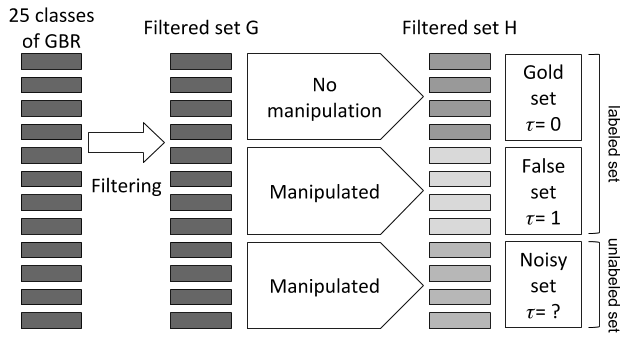
\includegraphics[width=\linewidth]{synthset}
\caption{Obtaining set $G$ and set $H$.}
\label{fig1}
\end{figure}

					%%%%%%%%%%
					\subsection{Experimental settings}
					\label{section:settings}
					%%%%%%%%%%



We aim to test the performance of the algorithm in different settings. The manipulations in set $H$ are varied with respect to: 1) how representative the error-patterns in the labeled set are for the error-pattern in the noisy set, 2) the size of the labeled set, 3) the percentage of errors in the noisy set, and 4) the type of errors. 

Firstly, the error patterns in the labeled and noisy set could be generated such that they are similar, i.e. cases with certain characteristics have errors. This is referred to as the 'informed labeled set'. An informed labeled set should make it easier for the model to find the erroneous cases in the noisy set. We also generate errors in the labeled set using only part of the enterprise characteristics, the 'limited labeled set'. Also, we can introduce random errors in the labeled set: 'random labeled set'. 

The size of the labeled set varies with 50, 100 or 150 cases per NACE code. The percentage of errors introduced in the noisy set varies with 5\%, 10\% or 15\%. Two types of errors are introduced: obvious and subtle errors. When an observed NACE code is manipulated, we vary how related the new, manipulated label is to the observed label. A NACE code that is changed to a non-related NACE code is an obvious error. A NACE code that is changed to a more similar, related NACE code is a subtle error.

Moreover, the proposed model, including a machine learning model and a logistic regression model, can be simplified. Fewer predictors can be used in the logistic regression, or the logistic regression could be replaced by simply including an average error probability. When an average error probability is included, we ignore that the noise might be non-random.

% Settings for the number of activities;
% A machine learning model provides us with a probability for every class. So far, in the discussion of the algorithm, only the first predicted class (top 1) is considered. Instead, also the three most likely classes can be considered (top 3). We want to account for the fact that an enterprise can have multiple activities and a website may be biased towards a related activity.

Table \ref{tab:table2} gives an overview of the experimental settings. 

\begin{table}[h]
\caption{\label{tab:table2}Experimental settings.}
\centering 
\begin{tabular}{ll}
\hline
\textbf{Dataset}               &                                                              \\ \hline
Representativity error-pattern & informed labeled set,                                         \\
                               & limited labeled set,                                          \\
                               & random labeled set                                           \\
Size labeled set               & 50 per class, 100 per class, 150 per class                                                \\
Percentage of errors           & 5\%, 10\%, 15\%                                              \\
Error type                     & obvious, subtle                                              \\ \hline
\textbf{Model}                 &                                                              \\ \hline
Modeling $\pi_i$               & logistic regression to estimate $\pi_i$,                      \\
                               & logistic regression (limited predictors) to estimate $\pi_i$, \\
                               & use a fixed, average error probability $\pi$                
\end{tabular}
\end{table}




					%%%%%%%%%%
					\subsection{Evaluation metrics}
					\label{section:evaluation}
					%%%%%%%%%%


% Evaluate which of the NACE codes are predicted to be erroneous

%% INCLUDE ACCURACY.

To evaluate the model performances, we investigate if the model indeed points out the manipulated cases in the noisy set as erroneous and estimates the non-manipulated cases in the noisy set as correct. 

In a confusion matrix we find the number true positives (TP), false positives (FP), true negatives (TN) and false negatives (FN). The predicted value for $z_i$ is compared with the observed value for $z_i$. With the confusion matrix, the precision, recall and accuracy are computed. 

Furthermore, we look at the cross-entropy loss, also called log loss. The cross-entropy loss is defined on the probability estimates for $z_i$, that are given by $\tau_i$. The cross-entropy loss takes the uncertainty of the predicted labels into account. The further the value of the log loss deviates from 0, the further away the predicted probability is from the actual class. The loss function takes the average of all individual cross-entropies:
						
						\begin{equation}\label{logloss}
- \frac{1}{N} \sum_i z_i log(p_i) + (1-z_i) log (1-p_i),
						\end{equation}

%http://wiki.fast.ai/index.php/Log_Loss

where $N$ is the total number of enterprises. Further, $z_i$ is the true label and indicates either an erroneous case or a correct case. Here $p_i = P(z_i=1) = \tau_i$, this denotes the estimated probability of being an erroneous case. 

\bigskip

					%%%%%%%%%%
					\subsection{Results}
					\label{section:resultsexp}
					%%%%%%%%%%

Here, the results of the experiments will be presented. We will discuss how the model performed under different circumstances. The best performing model(s) will be applied to the real-world data.

%% Application to real-world data
					%%%%%%%%%%
					\section{Application to real-world data}
					\label{section:application}
					%%%%%%%%%%

The model(s) will be implemented on the enterprises in the GBR.




\clearpage % to make sure references are on separate page

\bibliographystyle{apacite} 
\bibliography{references_VO}

\end{document}

